\section{\textbf{Use cases}}

\begin{figure}[H]
    \centering
    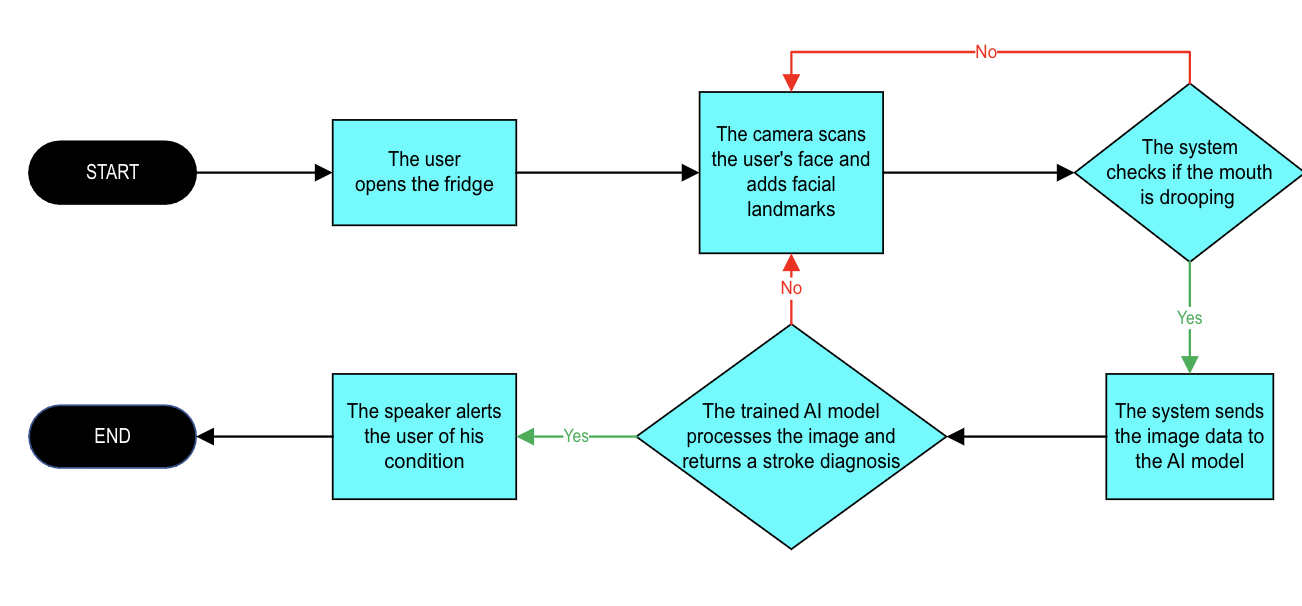
\includegraphics[width=1\linewidth]{images/use_cases.png}
    \caption{Use cases}
    \label{fig:use_cases}
\end{figure}

\subsection{\textbf{Use Case 1 : The user opens the fridge}}

\begin{figure}[H]
    \centering
    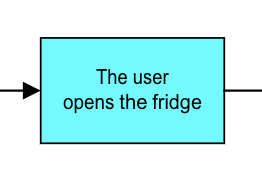
\includegraphics[width=0.33\linewidth]{images/use_case1.png}
    \caption{Use case 1}
    \label{fig:use_case1}
\end{figure}

The user goes to the refrigerator, that is equipped with a built in camera, connected to a Raspberry Pi.

\subsection{\textbf{Use Case 2 : The camera scans the user's face and adds facial landmarks}}

\begin{figure}[H]
    \centering
    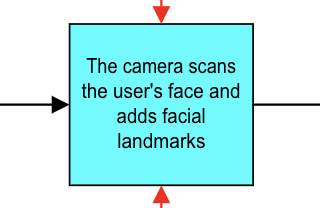
\includegraphics[width=0.33\linewidth]{images/use_case2.png}
    \caption{Use case 2}
    \label{fig:use_case2}
\end{figure}

\begin{figure}[H]
    \centering
    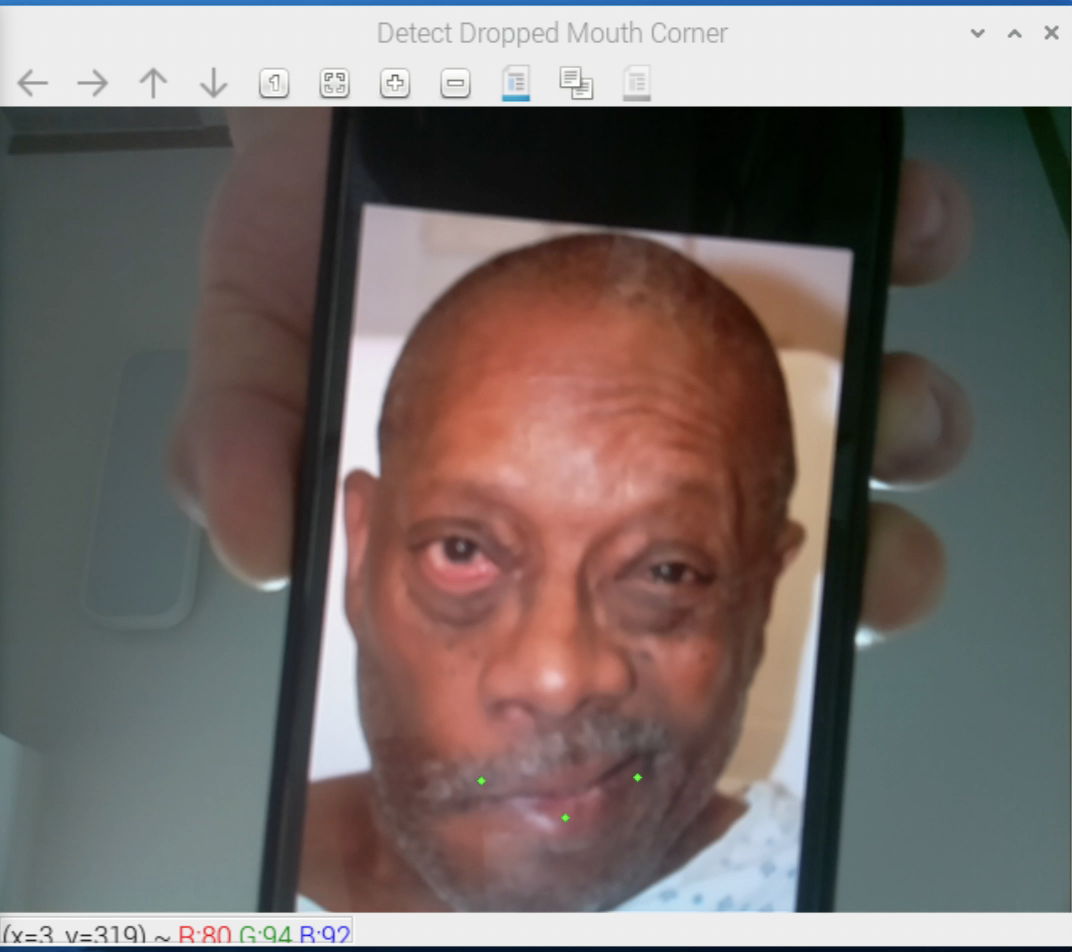
\includegraphics[width=0.5\linewidth]{images/Image.png}
    \caption{Image and facial landmarks}
    \label{fig:image and facial landmarks}
\end{figure}

This is the first level detection. The camera checks for mouth drooping in real time as long as the refrigerator is still open. The process runs offline on the local device for privacy concerns. 

\subsection{\textbf{Use Case 3 : The system checks if the mouth is drooping}}

\begin{figure}[H]
    \centering
    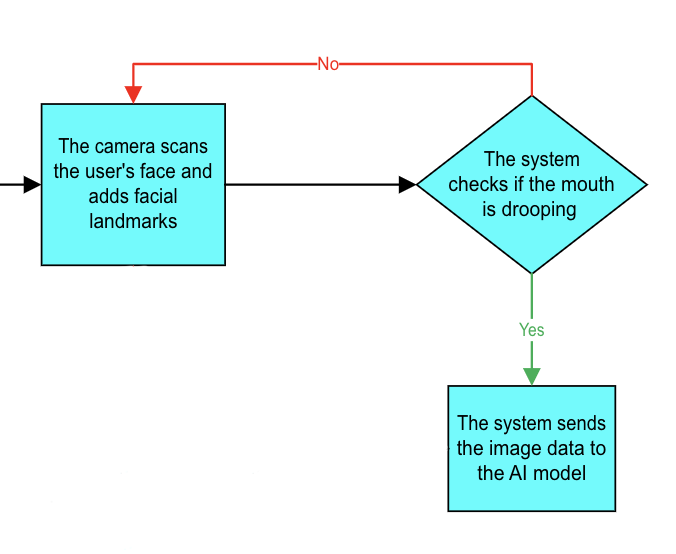
\includegraphics[width=0.7\linewidth]{images/use_case3.png}
    \caption{Use case 3}
    \label{fig:use_case3}
\end{figure}

\begin{figure}[H]
    \centering
    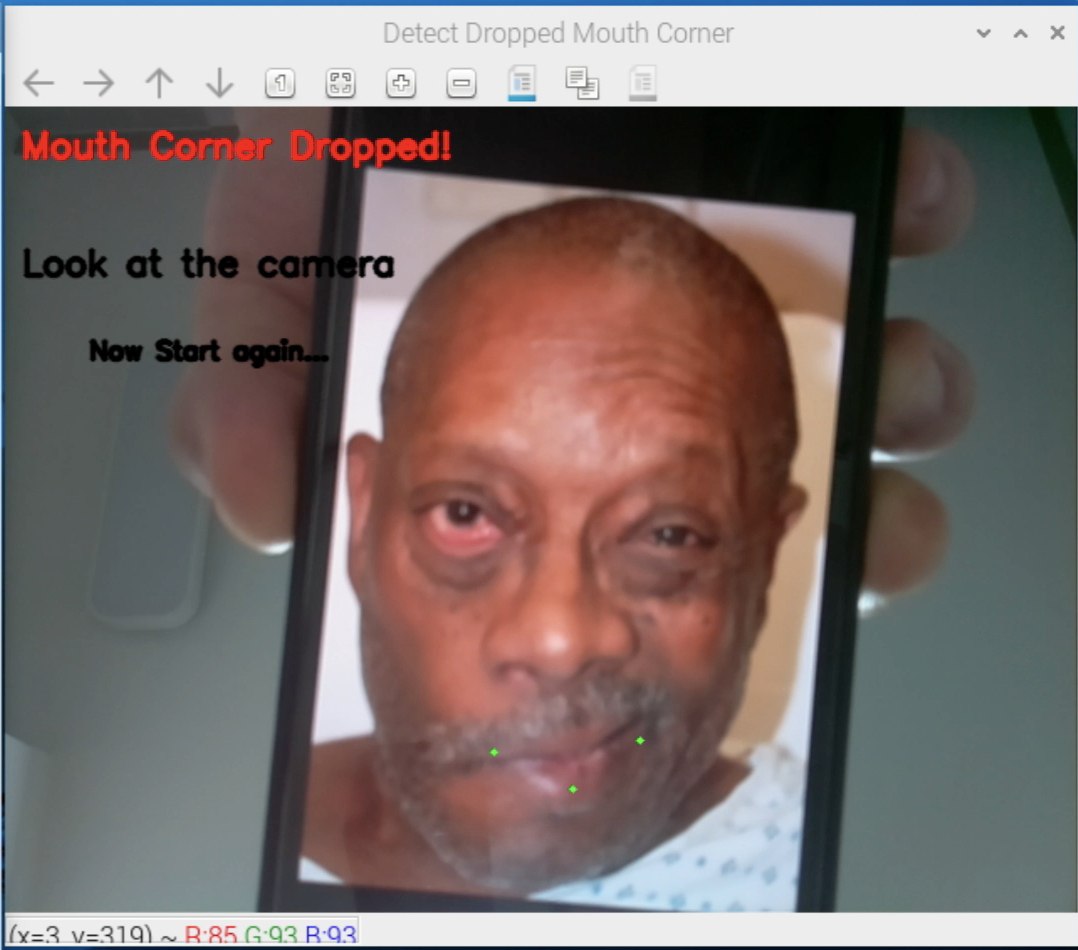
\includegraphics[width=0.5\linewidth]{images/Drooping detected.png}
    \caption{Mouth drooping}
    \label{fig:mouth drooping}
\end{figure}

\begin{figure}[H]
    \centering
    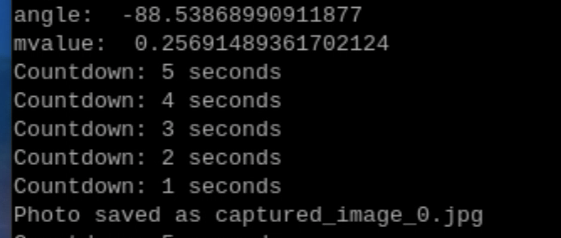
\includegraphics[width=0.7\linewidth]{images/Take picture.png}
    \caption{Picture taken}
    \label{fig:picture taken}
\end{figure}

When the camera detects the facial landmarks of the user's face, it calculates the m-value which is a value that correlate a renown symptom of stroke. If the m-value is under 0.25, nothing happens and the images taken aren't saved. However, when the m-value goes above 0.25, a more accurate picture is taken and the image data is sent to the AI model for processing.

\subsection{\textbf{Use Case 4 : The system sends the image data to the AI model}}

\begin{figure}[H]
    \centering
    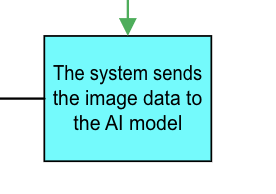
\includegraphics[width=0.33\linewidth]{images/use_case4.png}
    \caption{Use case 4}
    \label{fig:use_case4}
\end{figure}

Since the accuracy of the first level detection is low, we move to the second level detection. When the first level detection is triggered, the system establishes a connection with the server to send the image for further detection by a trained artificial intelligence model.

\subsection{\textbf{Use Case 5 : The trained AI model processes the image and return a stroke diagnosis}}

\begin{figure}[H]
    \centering
    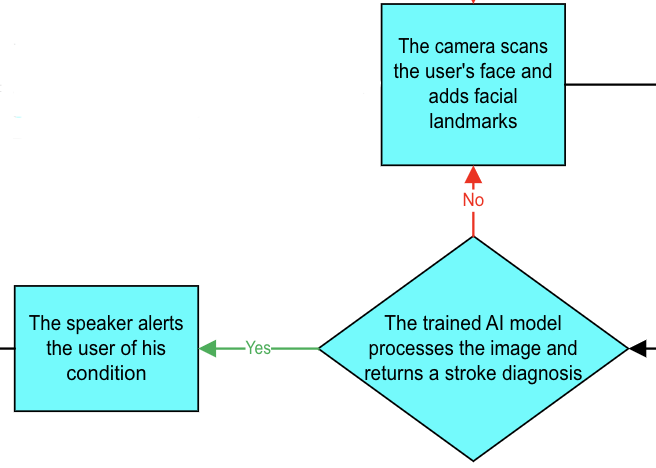
\includegraphics[width=0.7\linewidth]{images/use_case5.png}
    \caption{Use case 5}
    \label{fig:use_case5}
\end{figure}

\begin{figure}[H]
    \centering
    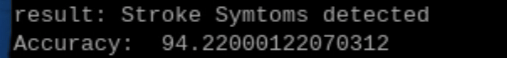
\includegraphics[width=1\linewidth]{images/Result.png}
    \caption{Result}
    \label{fig:result}
\end{figure}

The image received from the Raspberry Pi is verified by the AI model. The return value is 1 for a positive stroke prognostic and 0 for a negative stroke prognostic; the probability of each value is returned also.

\subsection{\textbf{Use Case 6 : The speaker alerts the user of his condition}}

\begin{figure}[H]
    \centering
    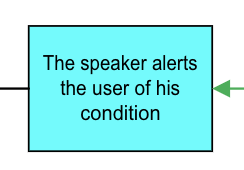
\includegraphics[width=0.33\linewidth]{images/use_case6.png}
    \caption{Use case 6}
    \label{fig:use_case6}
\end{figure}

If the diagnosis indicates the absence of a stroke, the system continues its operation without any specific signals. However, if the diagnosis indicates a high possibility of a stroke, the user is promptly informed of his condition and a step-by-step series of actions to do is given as advice to the user in order to stay safe.